
\documentclass[tikz,convert={convertexe={magick.exe}}]{standalone}
%\documentclass[tikz,convert]{standalone}
\usetikzlibrary{arrows}

\usepackage{ifthen}

\usepackage{amssymb}
\newcommand{\into}{\mathop{\lrcorner}}

\usetikzlibrary{snakes}
\usetikzlibrary{decorations.pathmorphing}

\begin{document}
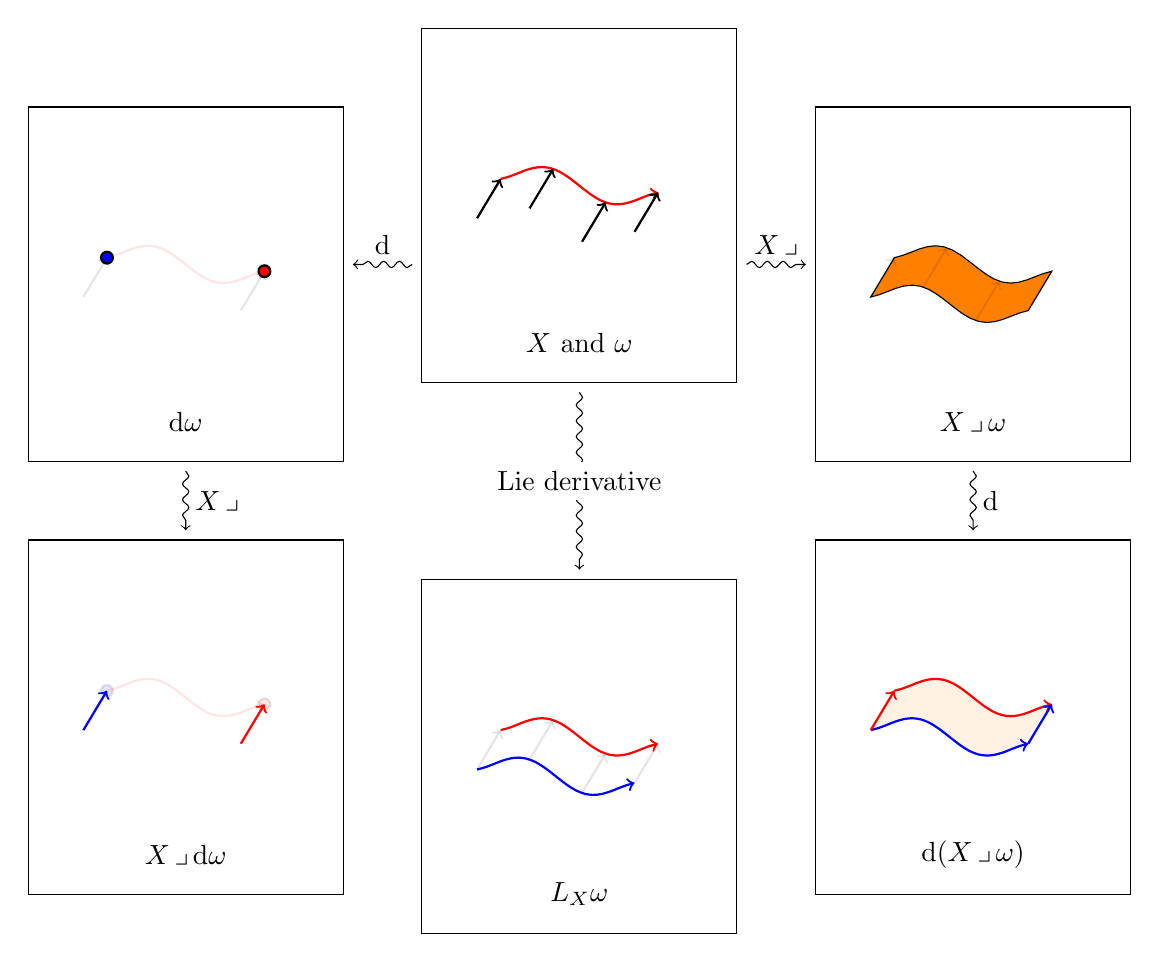
\begin{tikzpicture}

\tikzstyle atom=[circle, draw, inner sep=1.2pt, fill=red, thick]
\tikzstyle bigatom=[circle, draw, inner sep=1.5pt, fill=red, thick]
\tikzstyle snakearrow=[->,decorate,decoration={snake,amplitude=.4mm,segment length=2mm,post length=1mm}]

\begin{scope}[yshift=1cm]

\draw (-2,-2.5) rectangle (2,2);
\node at (0,-2) {$X$ and $\omega$};

\draw[red, thick,->] plot[smooth] coordinates{(-1.000,0.086) (-0.895,0.115) (-0.789,0.155) (-0.684,0.196) (-0.579,0.226) (-0.474,0.237) (-0.368,0.223) (-0.263,0.183) (-0.158,0.120) (-0.053,0.042) (0.053,-0.042) (0.158,-0.120) (0.263,-0.183) (0.368,-0.223) (0.474,-0.237) (0.579,-0.226) (0.684,-0.196) (0.789,-0.155) (0.895,-0.115) (1.000,-0.086)};
\draw[->,thick] (-1.300,-0.414)--(-1.000,0.086);
\draw[->,thick] (-0.633,-0.288)--(-0.333,0.212);
\draw[->,thick] (0.033,-0.712)--(0.333,-0.212);
\draw[->,thick] (0.700,-0.586)--(1.000,-0.086);

\node (XS) at (0,-2.5) {};
\node (XE) at (2,-1) {};
\node (XW) at (-2,-1) {};
\end{scope}

\begin{scope}[yshift=-6cm]

\draw (-2,-2.5) rectangle (2,2);
\node at (0,-2) {$L_X \omega$};

\draw[red, thick,->] plot[smooth] coordinates{(-1.000,0.086) (-0.895,0.115) (-0.789,0.155) (-0.684,0.196) (-0.579,0.226) (-0.474,0.237) (-0.368,0.223) (-0.263,0.183) (-0.158,0.120) (-0.053,0.042) (0.053,-0.042) (0.158,-0.120) (0.263,-0.183) (0.368,-0.223) (0.474,-0.237) (0.579,-0.226) (0.684,-0.196) (0.789,-0.155) (0.895,-0.115) (1.000,-0.086)};
\draw[blue, thick,->] plot[smooth] coordinates{(-1.300,-0.414) (-1.195,-0.385) (-1.089,-0.345) (-0.984,-0.304) (-0.879,-0.274) (-0.774,-0.263) (-0.668,-0.277) (-0.563,-0.317) (-0.458,-0.380) (-0.353,-0.458) (-0.247,-0.542) (-0.142,-0.620) (-0.037,-0.683) (0.068,-0.723) (0.174,-0.737) (0.279,-0.726) (0.384,-0.696) (0.489,-0.655) (0.595,-0.615) (0.700,-0.586)};
\draw[->,thick,opacity=0.1] (-1.300,-0.414)--(-1.000,0.086);
\draw[->,thick,opacity=0.1] (-0.633,-0.288)--(-0.333,0.212);
\draw[->,thick,opacity=0.1] (0.033,-0.712)--(0.333,-0.212);
\draw[->,thick,opacity=0.1] (0.700,-0.586)--(1.000,-0.086);

\node (LXWN) at (0,2) {};
\node (LXWW) at (-2,0) {};
\end{scope}

\begin{scope}[xshift=5cm]
\draw (-2,-2.5) rectangle (2,2);
\node at (0,-2) {$X \into \omega$};
\draw[draw=black, fill=orange] (-1.000,0.086)--(-0.895,0.115)--(-0.789,0.155)--(-0.684,0.196)--(-0.579,0.226)--(-0.474,0.237)--(-0.368,0.223)--(-0.263,0.183)--(-0.158,0.120)--(-0.053,0.042)--(0.053,-0.042)--(0.158,-0.120)--(0.263,-0.183)--(0.368,-0.223)--(0.474,-0.237)--(0.579,-0.226)--(0.684,-0.196)--(0.789,-0.155)--(0.895,-0.115)--(1.000,-0.086)--(0.700,-0.586)--(0.595,-0.615)--(0.489,-0.655)--(0.384,-0.696)--(0.279,-0.726)--(0.174,-0.737)--(0.068,-0.723)--(-0.037,-0.683)--(-0.142,-0.620)--(-0.247,-0.542)--(-0.353,-0.458)--(-0.458,-0.380)--(-0.563,-0.317)--(-0.668,-0.277)--(-0.774,-0.263)--(-0.879,-0.274)--(-0.984,-0.304)--(-1.089,-0.345)--(-1.195,-0.385)--(-1.300,-0.414)--cycle;
\draw[->,thick,opacity=0.1] (-1.300,-0.414)--(-1.000,0.086);
\draw[->,thick,opacity=0.1] (-0.633,-0.288)--(-0.333,0.212);
\draw[->,thick,opacity=0.1] (0.033,-0.712)--(0.333,-0.212);
\draw[->,thick,opacity=0.1] (0.700,-0.586)--(1.000,-0.086);

\node (YS) at (0,-2.5) {};
\node (YE) at (2,0) {};
\node (YW) at (-2,0) {};
\node (XIWS) at (0,-2.5) {};
\node (XIWW) at (-2,0) {};
\end{scope}

\begin{scope}[xshift=5cm,yshift=-5.5cm]
\draw (-2,-2.5) rectangle (2,2);
\node at (0,-2) {$\mathrm{d}(X \into \omega)$};
\draw[draw=none, fill=orange,opacity=0.1] (-1.000,0.086)--(-0.895,0.115)--(-0.789,0.155)--(-0.684,0.196)--(-0.579,0.226)--(-0.474,0.237)--(-0.368,0.223)--(-0.263,0.183)--(-0.158,0.120)--(-0.053,0.042)--(0.053,-0.042)--(0.158,-0.120)--(0.263,-0.183)--(0.368,-0.223)--(0.474,-0.237)--(0.579,-0.226)--(0.684,-0.196)--(0.789,-0.155)--(0.895,-0.115)--(1.000,-0.086)--(0.700,-0.586)--(0.595,-0.615)--(0.489,-0.655)--(0.384,-0.696)--(0.279,-0.726)--(0.174,-0.737)--(0.068,-0.723)--(-0.037,-0.683)--(-0.142,-0.620)--(-0.247,-0.542)--(-0.353,-0.458)--(-0.458,-0.380)--(-0.563,-0.317)--(-0.668,-0.277)--(-0.774,-0.263)--(-0.879,-0.274)--(-0.984,-0.304)--(-1.089,-0.345)--(-1.195,-0.385)--(-1.300,-0.414)--cycle;

\draw[red, thick,->] plot[smooth] coordinates{(-1.000,0.086) (-0.895,0.115) (-0.789,0.155) (-0.684,0.196) (-0.579,0.226) (-0.474,0.237) (-0.368,0.223) (-0.263,0.183) (-0.158,0.120) (-0.053,0.042) (0.053,-0.042) (0.158,-0.120) (0.263,-0.183) (0.368,-0.223) (0.474,-0.237) (0.579,-0.226) (0.684,-0.196) (0.789,-0.155) (0.895,-0.115) (1.000,-0.086)};
\draw[blue, thick,->] plot[smooth] coordinates{(-1.300,-0.414) (-1.195,-0.385) (-1.089,-0.345) (-0.984,-0.304) (-0.879,-0.274) (-0.774,-0.263) (-0.668,-0.277) (-0.563,-0.317) (-0.458,-0.380) (-0.353,-0.458) (-0.247,-0.542) (-0.142,-0.620) (-0.037,-0.683) (0.068,-0.723) (0.174,-0.737) (0.279,-0.726) (0.384,-0.696) (0.489,-0.655) (0.595,-0.615) (0.700,-0.586)};
\draw[->,thick,red] (-1.300,-0.414)--(-1.000,0.086);
\draw[->,thick,blue] (0.700,-0.586)--(1.000,-0.086);

\node (DXIWN) at (0,2) {};
\end{scope}

\begin{scope}[xshift=-5cm]
\draw (-2,-2.5) rectangle (2,2);
\node at (0,-2) {$\mathrm{d} \omega$};
\draw[red, thick,->,opacity=0.1] plot[smooth] coordinates{(-1.000,0.086) (-0.895,0.115) (-0.789,0.155) (-0.684,0.196) (-0.579,0.226) (-0.474,0.237) (-0.368,0.223) (-0.263,0.183) (-0.158,0.120) (-0.053,0.042) (0.053,-0.042) (0.158,-0.120) (0.263,-0.183) (0.368,-0.223) (0.474,-0.237) (0.579,-0.226) (0.684,-0.196) (0.789,-0.155) (0.895,-0.115) (1.000,-0.086)};

\draw[->,thick,opacity=0.1] (-1.300,-0.414)--(-1.000,0.086);
\draw[->,thick,opacity=0.1] (0.700,-0.586)--(1.000,-0.086);

\node[bigatom,fill=blue] at (-1.000,0.086) {};
\node[bigatom] at (1.000,-0.086) {};


\node (DWS) at (0,-2.5) {};
\node (DWE) at (2,0) {};
\end{scope}

\begin{scope}[xshift=-5cm,yshift=-5.5cm]
\draw (-2,-2.5) rectangle (2,2);
\node at (0,-2) {$X \into \mathrm{d} \omega$};

\draw[red, thick,->,opacity=0.1] plot[smooth] coordinates{(-1.000,0.086) (-0.895,0.115) (-0.789,0.155) (-0.684,0.196) (-0.579,0.226) (-0.474,0.237) (-0.368,0.223) (-0.263,0.183) (-0.158,0.120) (-0.053,0.042) (0.053,-0.042) (0.158,-0.120) (0.263,-0.183) (0.368,-0.223) (0.474,-0.237) (0.579,-0.226) (0.684,-0.196) (0.789,-0.155) (0.895,-0.115) (1.000,-0.086)};

\node[bigatom,fill=blue,opacity=0.1] at (-1.000,0.086) {};
\node[bigatom,opacity=0.1] at (1.000,-0.086) {};

\draw[->,thick,blue] (-1.300,-0.414)--(-1.000,0.086);
\draw[->,thick,red] (0.700,-0.586)--(1.000,-0.086);



\node (XIDWN) at (0,2) {};
\node (XIDWE) at (2,0) {};
\end{scope}

\draw[snakearrow] (XS) -- (LXWN) node[midway, fill=white] {Lie derivative};
\draw[snakearrow] (XE) -- (XIWW) node[midway, above] {$X \into$};
\draw[snakearrow] (XIWS) -- (DXIWN) node[midway, right] {$\mathrm{d}$};
\draw[snakearrow] (XW) -- (DWE) node[midway, above] {$\mathrm{d}$};
\draw[snakearrow] (DWS) -- (XIDWN) node[midway, right] {$X \into$};

\end{tikzpicture}
\end{document}